
\section{Cost of Money}\label{sec:cost-of-money}

In the previous sections, we assumed that the cost of borrowing money is free.
In this section we incorporate the cost (interest and collateral) of borrowing money into our model.
For the flash loan, the adversary must pay an extra
$\betaasset b$ \asset in fees upon returning the borrowed $b$ \asset.
The adversary must also pay interest on the $z$ \stasset she borrowed.
The duration of the loan was $\Delta_z = t_5 - t_0$, so the
total loan amount to be repaid, including the principal and interest, is
$((1 + \rstasset)^{\Delta_z} + \betastasset) z$ \stasset.
Letting $f = ((1 + \rstasset)^{\Delta_z} + \betastasset)$ be the cost factor
of the loan, to recover this amount of \stasset and pay back the loan, the adversary must now
deposit $b' = \frac{b_0}{s_0}(1 - p\frac{b}{b_0 + b}) f z$ \asset
into the protocol instead of $\frac{b_0}{s_0}(1 - p\frac{b}{b_0 + b}) z$ \asset like before.

Additionally, loans must be overcollateralized.
Let $\gammastasset$ be the collateral ratio of a standard \stasset loan.
The adversary, using her initial capital $u$ as collateral can get a loan of
up to $z = \frac{u}{\gammastasset} \frac{s_0}{b_0}$ \stasset
instead of the previous $u \frac{s_0}{b_0}$ \stasset.
The loaned $z$ \stasset are then converted to $b^*=\frac{u}{\gammastasset}$ \asset.
To perform the attack, part of the $b^*$ \asset is used to exempt delegate $c$ like
before, but another part is now used to pay $\betaasset b$ for the flash loan cost.
Hence $c + \betaasset b \leq b^*$ and the adversary may only use up to
$b \leq \frac{u}{(\frac{1}{\phi} + \betaasset) \gammastasset}$ to move the price
of \stasset.


Taking into consideration the cost of borrowing money, the final profit of the attack is now
$\alpha = b^* - b' - qc - \betaasset b$ for the new values of $b^*$ and $b'$.
Solving for $\frac{d\alpha}{db} = 0$ gives the optimal
$b = \sqrt{\frac{u f p b_0}{(\betaasset + \frac{q}{\phi})\gammastasset}} - b_0$,
which maximizes the adversary's profit, subject to the new constraints
$0 \leq b \leq \frac{u}{(\frac{1}{\phi} + \betaasset) \gammastasset}$.
Solving the inequality $\alpha \leq 0$ for $\frac{\phi}{q}$ and plugging in the adversarially optimal value for $b$
yields the new parametrization that renders the protocol secure

\begin{gather*}
  \frac{\phi}{q} \leq \frac{b_0 \gammastasset}{f p u + f u - b_0 \betaasset \gammastasset - 2 u \sqrt{fp (f-1)} - u}\,.
\end{gather*}

The cost of borrowing money increases when the collateral ratio
$\gammastasset$, the flash loan cost factor $\betaasset$ or the loan cost factor $f$
increase. While the cost of borrowing money goes up, the attack becomes less profitable
for the adversary. Thus, the protocol can afford to increase $\frac{\phi}{q}$
and still remain secure. The effect of varying $f$ is illustrated in
Figure~\ref{fig:plotf} for an adversary with $30\%$ and $50\%$ market domination $\frac{u}{b_0}$.
While $f$ increases, the safe bound of parameter $\frac{\phi}{q}$ can increase with it.
The black line indicates where the attack becomes unprofitable for the adversary ($\alpha = 0$).
The white area under the black line represents the configuration in which
the protocol is secure in the rational model.

\begin{figure*}[htb]
  \centering
  \ifccs
    \begin{subfigure}{0.4\textwidth}
  \fi
  \iflncs
    \begin{subfigure}{0.49\textwidth}
  \fi
    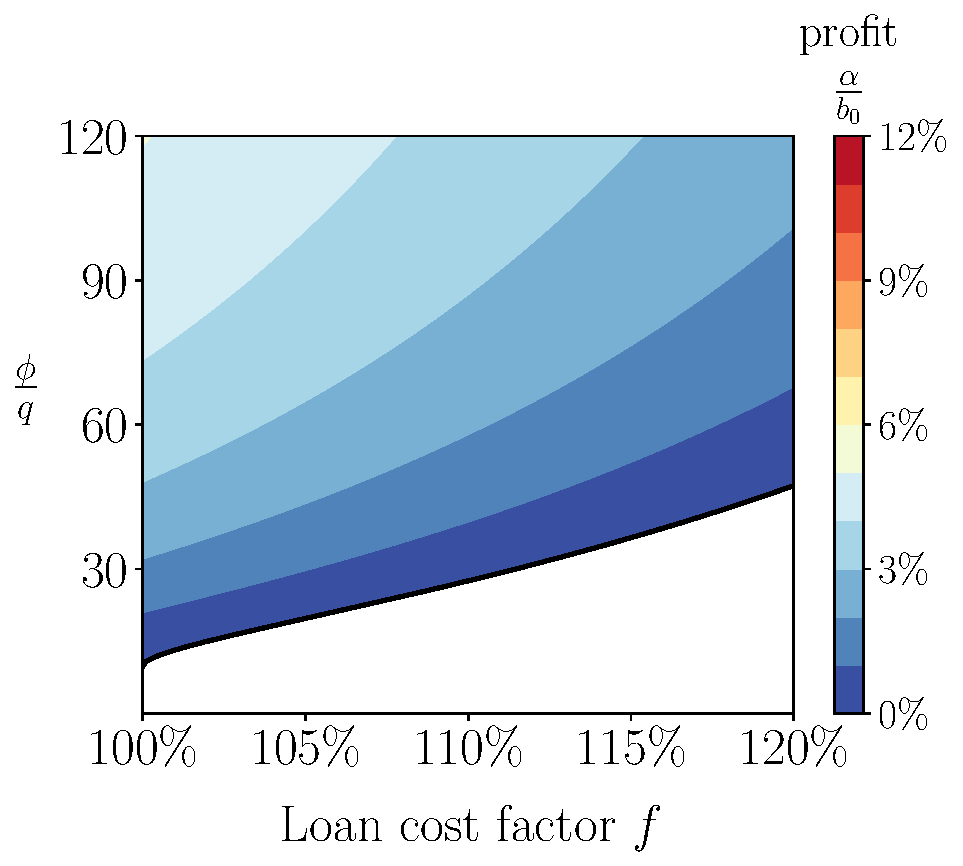
\includegraphics[width=\textwidth]{./figures/plotf30.pdf}
    \caption{Initial capital $u$ is $30\%$ of $b_0$.}
    \label{fig:plotf30}
  \end{subfigure}
  \ifccs
    \hspace{10mm}
    \begin{subfigure}{0.4\textwidth}
  \fi
  \iflncs
    \hfill
    \begin{subfigure}{0.49\textwidth}
  \fi
    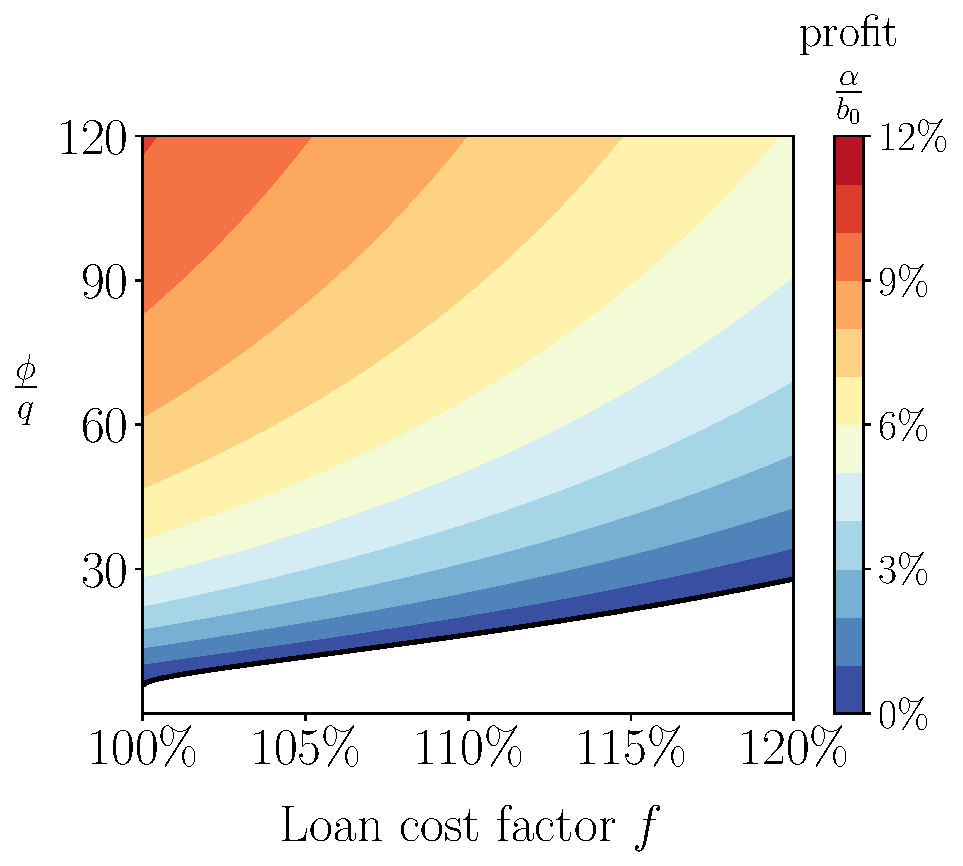
\includegraphics[width=\textwidth]{./figures/plotf50.pdf}
    \caption{Initial capital $u$ is $50\%$ of $b_0$.}
    \label{fig:plotf50}
  \end{subfigure}
  \caption{Cost of borrowing and attack profitability.}
  \label{fig:plotf}
\end{figure*}

In this illustration,
we consider a blockchain with slashing percentage
$p = 0.5$ and market conditions\footnote{\label{footnote:aave}ETH and Lido stETH borrowing rates
on Aave~\cite{aave} as of 27 Jan, 2023.}
with \asset flash loan cost factor $\betaasset = 0.09\%$ and
collateral ratio $\gammastasset = 146\%$.
At the time of writing\textsuperscript{\ref{footnote:aave}}, the annual cost of borrowing \stasset
is $\rstasset = 1.59\%$ (and $\betastasset = 0$ for non-flash loans).
If the attack duration is $\Delta_z = 20$ sec, we have
 $f = 1 + 10^{-8}$.
Hence, in practice, $f \simeq 1$, and money borrowing is almost free
for short durations.

Free money borrowing makes the adversary more powerful
and her attack more profitable.
Hence, a safe $\frac{\phi}{q}$ under free
borrowing ($f = 100\%$, $\betaasset = 0$, $\gammastasset = 100\%$)
is also safe when borrowing is not free.
This is illustrated in
Figure~\ref{fig:plotu}. Safe values of parameter $\frac{\phi}{q}$
for $f = 100\%$, indicated by the black line, are also safe for $f > 100\%$
under any adversarial market domination $\frac{u}{b_0}$.
Similarly, safe parametrizations for $\gammastasset = 100\%$ are also safe
for $\gammastasset > 100\%$.
We deduce that formula~(\ref{eq:phi-choice}) suffices for calculating
safe protocol parameters.

\begin{figure*}[htb]
  \centering
  \ifccs
    \begin{subfigure}{0.4\textwidth}
  \fi
  \iflncs
    \begin{subfigure}{0.49\textwidth}
  \fi
    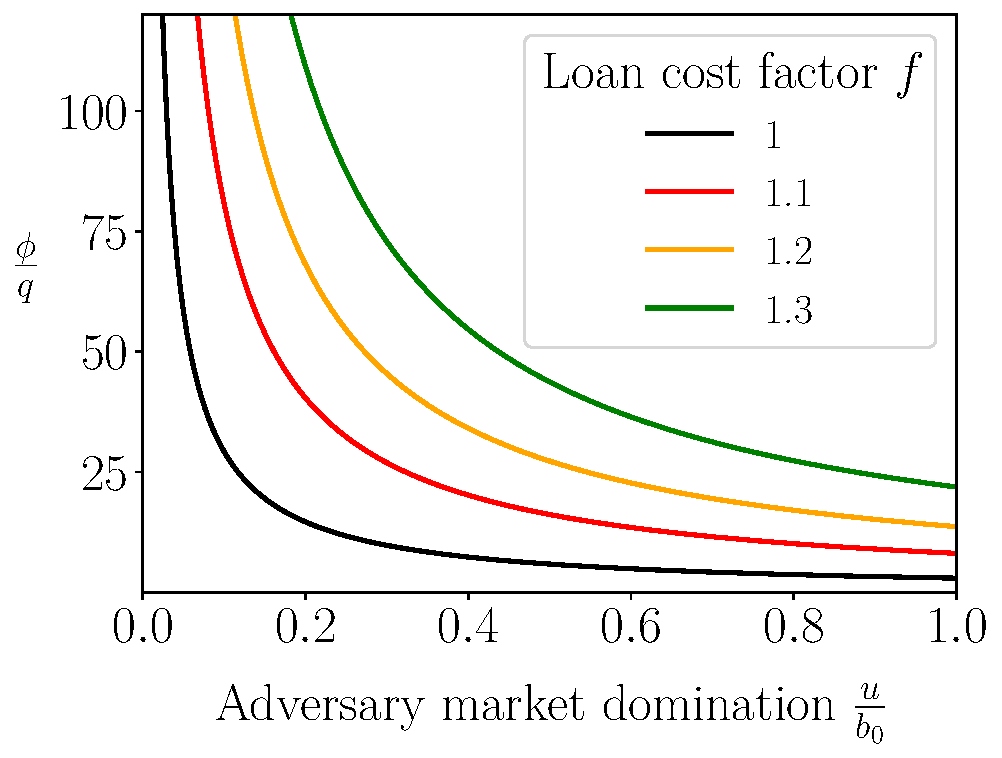
\includegraphics[width=\textwidth]{./figures/multiplef_plotu.pdf}
    \caption{For varying loan cost $f$.}
    \label{fig:compare-f-plotu}
  \end{subfigure}
  \ifccs
    \hspace{10mm}
    \begin{subfigure}{0.4\textwidth}
  \fi
  \iflncs
    \hfill
    \begin{subfigure}{0.49\textwidth}
  \fi
    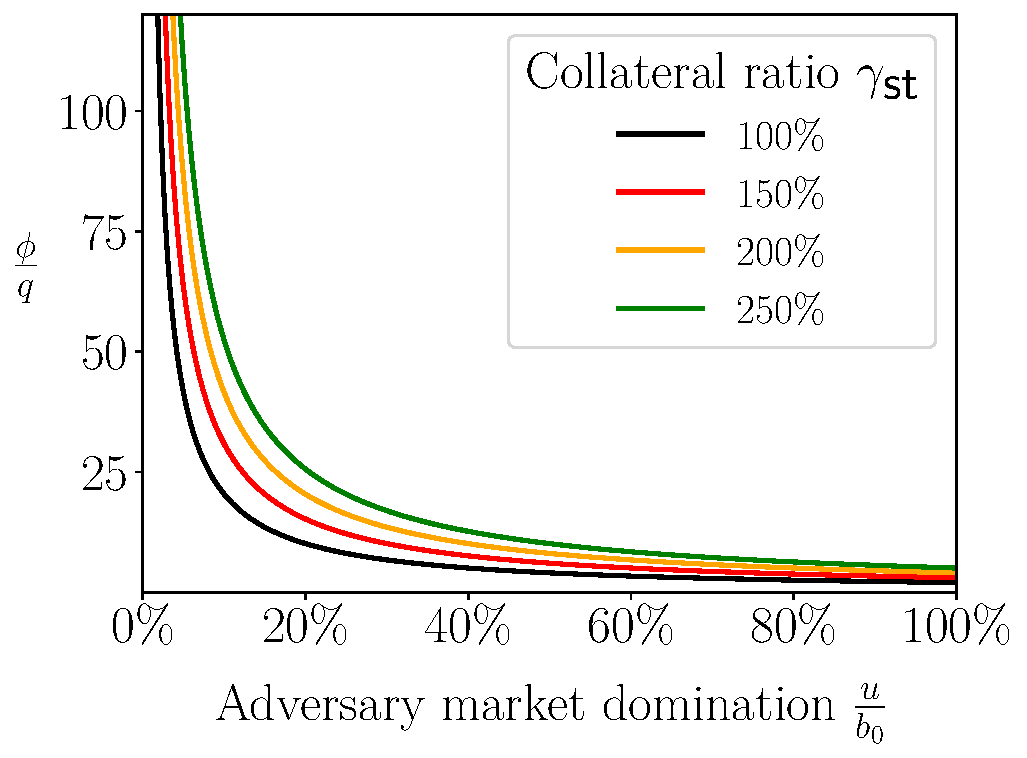
\includegraphics[width=\textwidth]{./figures/multiplegamma_plotu.pdf}
    \caption{For varying collateral ratio $\gamma$.}
    \label{fig:compare-f-plotu}
  \end{subfigure}
  \caption{Optimal $\frac{\phi}{q}$ for varying adversarial market domination
           $\frac{u}{b_0}$ and different market conditions.}
  \label{fig:plotu}
\end{figure*}



\noindent
\textbf{Bookkeeping in USD.}
If the attacker does bookkeeping in a different currency,
such as USD, the attack remains profitable. She begins by buying
\asset for USD. At the end of the attack, she sells \asset for USD.
Because the attack concerns a particular liquid staking protocol, and
not the whole \asset network, the price of \asset will likely not
be significantly affected.
This attack decreases the market confidence in \stasset,
but not in \asset.
In fact, because
the attack causes slashing of \asset, the supply of \asset is decreased
and the price of \asset with respect to the reference currency may
even increase.
Lastly, any price fluctuations of \asset with respect to USD will likely be
minor, as the attack has a short duration of a couple of seconds.

\noindent
\textbf{The Market price of \stasset.}\label{sec:stasset-price}
Let us consider the price $v$ of \stasset denominated in \asset in the market.

\emph{Upper bound.}
Because the option always exists to mint at a rate of $\frac{s_0}{b_0}$ by
depositing, the price of \stasset denominated in \asset in a perfectly
efficient market is $\frac{b_0}{s_0}$ at maximum. Otherwise, no
rational buyer would use the market. Hence, the market rate is
$v \leq \frac{b_0}{s_0}$.

\emph{Lower bound.}
There are two options to convert $s$ \stasset to \asset: either sell
at the market rate to obtain $b = v s$ \asset, or use the redemption mechanism.
Using the redemption mechanism, the \assets become available after
time $\delta$.
Initially, using $s$ \stasset, a redemption is made of $b' = s \frac{b_0}{s_0}$
delegated assets. To get $b$ \asset immediately (and avoid having to wait
for the unbonding period), a loan of $b$ \asset is taken~\cite[p.~13]{liquid-staking-report} and
repaid after duration $\delta$.
The amount of \asset that needs to be paid back,
including principal and interest, is $((1 + \rasset)^\delta + \betaasset)b$ \asset.
We set this amount to be equal to $b'$, the amount of \assets that will be
unbonded after $\delta$ time. Solving for $b$, we get
$b = s \frac{b_0}{s_0 ((1 + \rasset)^\delta + \betaasset)}$.
Therefore, in an efficient market $v \geq \frac{b_0}{s_0 ((1 + \rasset)^\delta + \betaasset)}$.

We deduce that the bounds for an efficient market of \asset and \stasset are

\[
  \frac{b_0}{s_0 ((1 + \rasset)^\delta + \betaasset)} \leq v \leq \frac{b_0}{s_0}\,.
\]

The longer the duration $\delta$, the larger the potential price deviation
(c.f. the empirical analysis in
\emph{Liquid Staking: Basis Determinants and Price Discovery}~\cite{scharnowski2022liquid}).
Such loans are available in practice and some
protocols~\cite[\S5]{parallel}\cite{marinade-matching} even automate this process.

It is also possible for the protocol to use the principle of \emph{remittances}
(matching)~\cite[\S5]{parallel}\cite{marinade-matching} to match depositing and
redeeming parties, so that the redeeming party does not have to incur any unbonding delay.
If the redeemed amounts exceed the deposited amounts, some amounts will necessarily incur
a delay. The above bounds may be tighter due to
a shorter effective unbonding delay.
